
% \documentclass[notes=show]{beamer}
\documentclass[xcolor=dvipsnames, xcolor=table, 10pt]{beamer}
%%%%%%%%%%%%%%%%%%%%%%%%%%%%%%%%%%%%%%%%%%%%%%%%%%%%%%%%%%%%%%%%%%%%%%%%%%%%%%%%%%%%%%%%%%%%%%%%%%%%%%%%%%%%%%%%%%%%%%%%%%%%%%%%%%%%%%%%%%%%%%%%%%%%%%%%%%%%%%%%%%%%%%%%%%%%%%%%%%%%%%%%%%%%%%%%%%%%%%%%%%%%%%%%%%%%%%%%%%%%%%%%%%%%%%%%%%%%%%%%%%%%%%%%%%%%

\usepackage{amsmath}
\usepackage{mathpazo}
\usepackage[authoryear]{natbib}             % Option: Use NatBib bibliography styles
\usepackage{hyperref}
\usepackage{multimedia}
\usepackage{graphicx}
\usepackage{helvet}
\usepackage[english]{babel}
\usepackage[latin1]{inputenc}
\usepackage{comment}
\usepackage{color}
\usepackage{epstopdf}
\usepackage{appendixnumberbeamer}
\usepackage{transparent}
\usepackage{xcolor}
\usepackage{relsize}
\usepackage{booktabs}
\usepackage{amsthm}
\usepackage{threeparttable, tablefootnote} % table footnote
\usepackage{PlayfairDisplay}

\DeclareMathOperator*{\argmin}{argmin} % thin space, limits underneath in displays
\usepackage{bbm}



\setcounter{MaxMatrixCols}{10}

% \useinnertheme{circles}
\usefonttheme{serif}
% \usecolortheme{orchid}

\usecolortheme[RGB={26,58,95}]{structure}
\beamertemplatenavigationsymbolsempty

\definecolor{orange}{RGB}{255,127,0}
\newcommand{\bb}[1]{{\color{euiblue}#1}}
\newcommand{\gre}[1]{{\color{applegreen}#1}}
\newcommand{\rr}[1]{{\color{darkred}#1}}
\newcommand{\orr}[1]{{\color{orange}#1}}
\definecolor{upf}{RGB}{192,0,37}
\definecolor{euiblue}{RGB}{56,136,199}
\definecolor{fedblue}{RGB}{26,58,95}
\definecolor{darkred}{rgb}{0.55, 0.0, 0.0}
\definecolor{applegreen}{rgb}{0.55, 0.71, 0.0}
\definecolor{orange}{rgb}{0.93, 0.53, 0.18}

\usepackage{mathtools}

 \newcommand{\lefta}{ \left[\begin{array} } 	
\newcommand{\righta}{ \end{array} \right]} 	

\newcommand*{\vcenterimage}[1]{\vcenter{\hbox{\includegraphics[width=0.35\linewidth]{#1}}}}
\newcommand*{\vcenterarrow}{\vcenter{\hbox{$\Longrightarrow$}}}

\makeatletter
\def\blfootnote{\gdef\@thefnmark{}\@footnotetext}
\makeatother


\useitemizeitemtemplate{%
    \raise1.5pt\hbox{\color{beamerstructure}$\bullet$}%
}
\usesubitemizeitemtemplate{%
    \small\raise1.5pt\hbox{\color{beamerstructure}$\bullet$}%
}
\usesubsubitemizeitemtemplate{%
    \raise1.5pt\hbox{\color{beamerstructure}$\circ$}%
}


\setbeamersize{text margin left=1.5em,text margin right=1.5em}
\setbeamertemplate{footline}[frame number]

\usetheme{boadilla}


\begin{document}

\playfair

\title[Growth-At-Risk Models]{\textbf{Growth-At-Risk Models\\ for the U.S. and the Foreign Economy Outlook}}
\thispagestyle{empty}
\author[Caldara, Cascaldi-Garcia, Cuba-Borda, Loria]{\textbf{Dario Caldara (IF)\\ Danilo Cascaldi-Garcia (IF)\\ Pablo Cuba-Borda (IF)\\ Francesca Loria (R\&S)}\\ \medskip \emph{Board of Governors of the Federal Reserve System}}

%\date[Class II - FOMC]{\emph{May 12, 2020}}
\date[May 12, 2020]{\emph{May 12, 2020}}

\maketitle

% \begin{frame}{Overview}
% \tableofcontents
% \end{frame}

\setcounter{framenumber}{0}

\begin{frame}{A Framework to Track Risks to the Outlook}
\vspace*{0.12in}
\begin{itemize}
    \item Staff developed GDP ``growth-at-risk" (G@R) models for the United States and the foreign economy.
    \medskip
    \begin{itemize}
        \item {\bb{Goal:}} Quantify risks to the outlook.
    \end{itemize}
    \bigskip    
    \item Design principles:
    \bigskip
    \begin{itemize}
        \item Forecast oriented (comparison to staff baseline projection).
        \medskip
        \item Use of \rr{real-time} macroeconomic and financial indicators.
        \medskip
        \item Common platform to track risks to domestic and foreign outlook.
    \end{itemize}
    \bigskip
    \item Updates posted on the interactive webpage of the model
    \medskip
    \item[] \url{https://spweb.frb.gov/sites/ifdocs/ifdocs/Growth-At-Risk\%20interactive\%20weekly\%20updates/interactive-memo.html}

\end{itemize}

\end{frame}


\begin{frame}{An Overview of ``Growth-at-Risk"}
\vspace*{0.12in}
\begin{itemize}
    \item Model the \rr{entire} distribution of future real GDP growth \rr{conditional on economic activity and financial conditions}.
    \bigskip
    \item Key result: (Conditional) mean and volatility are negatively correlated.\\    
    \begin{center}
        $\longrightarrow$ \rr{Growth-at-Risk}! 
    \end{center}
    % \medskip
    
    %     \begin{itemize}
    %         \item {\footnotesize High mean - Low volatility: Normal state}
    %         \medskip
    %         \item {\footnotesize Low mean - High volatility: Large downside risks} 
    %    \end{itemize}
\end{itemize}
\begin{figure}
    \includegraphics[width=0.85\linewidth,keepaspectratio=true]{Slides/Figures/univariatefull-VC.pdf}
\end{figure}

\end{frame}

% \begin{frame}{Modelling "Growth-at-Risk"}

% \begin{itemize}
%     \item GaR as negative correlation between mean and volatility is a very robust finding across modelling approaches:
%     \smallskip
%       \begin{enumerate}
%             \item \rr{Quantile regressions} (QR)
%             \medskip
%             \item \rr{Stochastic volatility VARs}
%             \medskip
%             \item Markov switching models
%             \medskip
%             \item  Conditionally heteroskedastic models
%         \end{enumerate}
%         \bigskip
%     \item Approaches vary in:
%     \smallskip
%         \begin{itemize}
%             \item Flexibility
%             \medskip
%             \item Robustness
%             \medskip
%             \item Computational burden
%             \medskip
%             \item Details of the results
%         \end{itemize}
% \end{itemize}

% \end{frame}

\begin{frame}{Plan of the Talk}

\begin{enumerate}
    \item Quantile Regressions
    \bigskip
    \item From Quantiles to Distributions
    \bigskip
    \item Other Applications
    \begin{enumerate}
    \smallskip
        \item Inflation-at-Risk
        \medskip
        % \item \rr{Canada?}
        % \medskip
        \item Comparison to Growth-at-Risk for Financial Stability
    \end{enumerate}
\bigskip
\item Final Remarks
\end{enumerate}

\end{frame}


\section{Quantile Regressions}
\begin{frame}[noframenumbering]
\thispagestyle{empty}
       \begin{center}
         \structure{\Huge {\color{black}{\insertsection}}}
       \end{center}
     \end{frame}

\frame{
\frametitle{Fixing Ideas: PDF and CDF}
\label{visualizing}
\vspace{0.25cm}

\begin{itemize}
\item Consider a variable $y$, with probability distribution function $f(y)$ and cumulative distribution function $F(y)$.

\begin{figure}[h!]
\includegraphics[width=0.45\textwidth]{Slides/Figures/PDF}
\includegraphics[width=0.45\textwidth]{Slides/Figures/CDF}
\end{figure}

\end{itemize}
}

\frame{
\frametitle{Fixing Ideas: Quantile Function}
\label{fixing}
\vspace{0.25cm}

\begin{itemize}
\item Quantile function (CQF) of $y$ is
\begin{equation*}
  \text{Q}_{\tau} (y) = F^{-1}_y\left(\tau\right),\ \tau \in (0,1).
\end{equation*}

\begin{figure}[h!]
\includegraphics[width=0.6\textwidth]{Slides/Figures/CDF_Q}
\end{figure}

\end{itemize}
% \hyperlink{conditional}{\beamerbutton{Conditional Quantiles}} 
}

\frame{
\frametitle{Fixing Ideas: Approximating the Quantile Function}
\label{fixing2}
\vspace{0.25cm}

\begin{itemize}
\item Quantile function (CQF) of $y$ is
\begin{equation*}
  \text{Q}_{\tau} (y) = F^{-1}_y\left(\tau\right),\ \tau \in (0,1).
\end{equation*}

\begin{figure}[h!]
\includegraphics[width=0.6\textwidth]{Slides/Figures/CDF_discrete.pdf}
\end{figure}

\end{itemize}
% \hyperlink{conditional}{\beamerbutton{Conditional Quantiles}} 
}


\frame{
\frametitle{Quantile Regressions}
\label{qr}
\vspace{0.25cm}

{\small
\begin{itemize}
\item Linear model for conditional quantile function
\begin{equation*}
\text{Q}_{\tau} (y_t| x_t) = x_t \theta_{\tau},\ \tau \in (0,1)
\end{equation*}
where quantile regression slopes solve
\begin{equation*}
\hspace{-0.2cm}  \theta_{\tau} = \argmin_{\theta_{\tau}\in\mathbb{R}^k} \sum_{t=1}^{T} \bigl[\rho_{\tau} \underbrace{\left(y_t -x_t \hat{\theta}_{\tau}\right)}_{\equiv u_t} \bigr]
\end{equation*}
and $\rho_{\tau}(u)$ is the \hyperlink{checkfct}{\beamerbutton{Check Function}}.
% = \mathbb{1}(u\leq 0) (1-\tau) u + \mathbb{1} (u >0) \tau u
\bigskip
\item Quantile regression \textbf{differs from OLS} in these dimensions:\medskip
\begin{enumerate}
	\item Minimizes the \emph{weighted} sum of \emph{absolute} (vs. squared) errors.\medskip
	\item Weights depend on error terms being above or below a quantile $\tau$.
\end{enumerate}
\bigskip
%   \item \textbf{Example} of linear relationship between quantiles and conditioning variables:
% \begin{equation*}
%   \hat{\text{Q}}_{\tau} (\Delta \bar{y}_{t+1,t+12}| x_t) = \hat{\alpha}_{\tau} + \hat{\beta}_{\tau} VXO_t + \hat{\gamma}_{\tau} ADS_t,\ \tau \in (0,1).
% \end{equation*}
\hyperlink{disadvantagesqr}{\beamerbutton{Advantages and Disadvantages}}
\end{itemize}
}
}

\frame{
\frametitle{Model and Data}
\label{modeldata}
\vspace{0.25cm}

{\small
\begin{itemize}
  \item Quantile regressions:
    \begin{equation*}
      \hat{\text{Q}}_{\tau} (\Delta {\bar{y}\ }^j_{t+1,t+12}| FF_t,  MF_{t}^{\ j}) = \hat{\alpha}_{\tau} + \hat{\beta}_{\tau} FF_t + \hat{\gamma}_{\tau} MF_t^{\ j},\ \tau \in (0,1),\ j = \{ U.S., F.E. \}
    \end{equation*}
    % \medskip
    \item Monthly data are constructed using a Dynamic Factor Model:
    \medskip
    \begin{enumerate}
        \item Average GDP growth between month $t+1$ and $t+12$ ( \rr{$\Delta {\bar{y}\ }^j_{t+1,t+12}$})
        \bigskip
    	\item Financial Factor (\rr{FF}) extracted from:\medskip
        	\begin{itemize}
        	    \item VXO; Excess Bond Premium; TED spread; CBill Spread.\medskip
        	   % \item CBOE S\&P100 Volatility Index (VXO); 3-month Libor rate minus Treasury Bill (TED spread); 3-month Financial commercial paper minus Treasury bill (CBILL); Excess Bond Premium (EBP)\medskip
        	\end{itemize}
    	\item United States and foreign macroeconomic factors (\rr{${MF\ }^j$}):
    	\medskip
        	\begin{itemize}
        	    \item Monthly growth rates of IP \& retail sales;
        	    \item Quarterly growth rates of real GDP;
        	    \item New Export Order component of the PMI survey;
        	    \item Initial unemployment insurance claims (United States MF only)
        	\end{itemize}
    \end{enumerate}
    \medskip
    \item \rr{Estimation} sample: 1986m1-2019m4 
\end{itemize}
\hyperlink{Hist}{\beamerbutton{Historical Data}}
}
}

% \frame{
% \frametitle{Model and Data}
% \label{modeldata}
% \vspace{0.25cm}

% {\small
% \begin{itemize}
%   \item Quantile regressions:
%     \begin{equation*}
%       \hat{\text{Q}}_{\tau} (\Delta {\bar{y}\ }^j_{t+1,t+12}| FF_t,  ADS_{t}^{\ j}) = \hat{\alpha}_{\tau} + \hat{\beta}_{\tau} FF_t + \hat{\gamma}_{\tau} ADS_t^{\ j},\ \tau \in (0,1),\ j = \{ U.S., F.E. \}
%     \end{equation*}
% % \item Fit flexible probability distribution on estimated conditional quantiles to approximate the predictive distribution of average future GDP growth (\rr{1-Year Horizon})

% % \item The framework has two steps (same as Adrian et al 2019, AER):
% % \begin{enumerate}
% %     \item Quantile regressions:
% %     \begin{equation*}
% %       \hat{\text{Q}}_{\tau} (\Delta \bar{y}_{t+1,t+12}| FF_t,  ADS_{t}^{\ j}) = \hat{\alpha}_{\tau} + \hat{\beta}_{\tau} FF_t + \hat{\gamma}_{\tau} ADS_t^{\ j},\ \tau \in (0,1),\ j = \{ U.S., F.E. \}
% %     \end{equation*}
% % \item Fit flexible probability distribution on estimated conditional quantiles to approximate the predictive distribution of average future GDP growth (\rr{1-Year Horizon})
% % \end{enumerate}

% \medskip
% \item Data:
% \medskip
% \begin{enumerate}
% \item Average GDP growth between month t+1 and t+12 (\rr{$\Delta {\bar{y}\ }^j_{t+1,t+12}$})
% \bigskip
% 	\item Financial Factor (\rr{FF}) extracted from:\medskip
% 	\begin{itemize}
% 	    \item VXO; Excess Bond Premium; TED spread; CBill Spread.\medskip
% 	   % \item CBOE S\&P100 Volatility Index (VXO); 3-month Libor rate minus Treasury Bill (TED spread); 3-month Financial commercial paper minus Treasury bill (CBILL); Excess Bond Premium (EBP)\medskip
% 	\end{itemize}
% 	\bigksip
% 	\item United States and Foreign real-time business condition index (\rr{${ADS\ }^j$}):
% 	\medskip
% 	\begin{itemize}
% 	    \item Monthly growth rates of IP \& retail sales;
% 	    \item Quarterly growth rates of real GDP;
% 	    \item NEO component of the PMI survey;
% 	    \item Initial unemployment insurance claims (United States ADS only)
% 	\end{itemize}
% \end{enumerate}
% \medskip
% \item \rr{Estimation} sample: 1986m1-2019m4 
% \end{itemize}
% \hyperlink{Hist}{\beamerbutton{Historical Data}}
% % \\
% % $\longrightarrow$ Last in-sample observation of future GDP growth in 2019:m4 based on data from 2019:m5 through 2020:m4.

% %   \item \textbf{Example} of linear relationship between quantiles and conditioning variables:
% % \begin{equation*}
% %   \hat{\text{Q}}_{\tau} (\Delta \bar{y}_{t+1,t+12}| x_t) = \hat{\alpha}_{\tau} + \hat{\beta}_{\tau} VXO_t + \hat{\gamma}_{\tau} ADS_t,\ \tau \in (0,1).
% % \end{equation*}

% % \hyperlink{Data}{\beamerbutton{Data \& Estimation}}

% }
% }


\frame{
\frametitle{Slopes of Conditional Quantiles - United States}
\label{linearqr}
\begin{figure}[h!]
\begin{center}
{\scriptsize{Note: Black circles indicate observation pairs after December 2007.}}\\
 \includegraphics[width=0.45\textwidth]{Slides/Figures/slope_fin___Country=US___GDP=GDP___SpecWith=fin_ads___Scenario=Baseline___Lags=0___Sample=1986-Jan_to_2020-Apr.pdf}
 \includegraphics[width=0.45\textwidth]{Slides/Figures/slope_ads___Country=US___GDP=GDP___SpecWith=fin_ads___Scenario=Baseline___Lags=0___Sample=1986-Jan_to_2020-Apr.pdf}
% \includegraphics[width=0.3\textwidth]{Slides/Figures/slope_fin___Country=Foreign_TW___GDP=GDP___SpecWith=fin_ads___Scenario=Baseline___Lags=0___Sample=1986-Jan_to_2020-Apr.pdf}
%  \includegraphics[width=0.3\textwidth]{Slides/Figures/slope_ads___Country=Foreign_TW___GDP=GDP___SpecWith=fin_ads___Scenario=Baseline___Lags=0___Sample=1986-Jan_to_2020-Apr.pdf}
 \end{center}
\end{figure}
\begin{itemize}
\small
    \item \textbf{Key takeaway}: Lower quantile moves more than median and upper quantile \\ FF $\uparrow$ or MF $\downarrow$ $\rightarrow$ \rr{Rise in volatility and skewness of GDP}.
    % \medskip
    % \begin{enumerate}
    %     \item OLS and median are different (asymmetry).
    %     \medskip
    %     \item 
    % \end{enumerate}
 
\end{itemize}

}

\frame{
\frametitle{Slopes of Conditional Quantiles - Foreign Economy}
\begin{figure}[h!]
\begin{center}
{\scriptsize{Note: Black circles indicate observation pairs after December 2007.}}\\
%  \includegraphics[width=0.3\textwidth]{Slides/Figures/slope_fin___Country=US___GDP=GDP___SpecWith=fin_ads___Scenario=Baseline_AR_FF4___Lags=0___Sample=1986-Jan_to_2020-Apr.pdf}
%  \includegraphics[width=0.3\textwidth]{Slides/Figures/slope_ads___Country=US___GDP=GDP___SpecWith=fin_ads___Scenario=Baseline_AR_FF4___Lags=0___Sample=1986-Jan_to_2020-Apr.pdf}\\
\includegraphics[width=0.45\textwidth]{Slides/Figures/slope_fin___Country=Foreign_TW___GDP=GDP___SpecWith=fin_ads___Scenario=Baseline___Lags=0___Sample=1986-Jan_to_2020-Apr.pdf}
 \includegraphics[width=0.45\textwidth]{Slides/Figures/slope_ads___Country=Foreign_TW___GDP=GDP___SpecWith=fin_ads___Scenario=Baseline___Lags=0___Sample=1986-Jan_to_2020-Apr.pdf}
 \end{center}
\end{figure}
\begin{itemize}
\small
    \item \textbf{Key takeaways}:
    \medskip
    \begin{enumerate}
        \item FF: Lower and \emph{upper} quantiles move more than median. \\ $\longrightarrow$\rr{Rise in volatility of GDP}.
        \medskip
        \item MF: All quantiles move similarly.
        \\ $\longrightarrow$\rr{Location shift in GDP}.
    \end{enumerate}
 
\end{itemize}

}

\frame{
\frametitle{Obtaining the Time Series of Conditional Quantiles}
\vspace{0.5cm}

\begin{itemize}

\item At each point in time $t$, it is possible to use data on $FF_t$ and $MF_t$ to construct $\hat{\text{Q}}_{\tau} (\Delta \bar{y}_{t+1,t+12}| x_t)$.
\bigskip
\item \rr{Example}: Foreign Economy April 2020, $FF_{20:m4}=2.41$; $MF_{20:m4}=-6.85$.
  \bigskip
\begin{equation*}
      \hat{\text{Q}}_{\tau} (\Delta {\bar{y}}_{20:m5,21:m4}| FF_{20:m4},  MF_{20:m4}) = \hat{\alpha}_{\tau} + \hat{\beta}_{\tau} FF_{20:m4} + \hat{\gamma}_{\tau} MF_{20:m4}
    \end{equation*}
 \end{itemize}
 
 \begin{figure}[h!]
\includegraphics[width=0.5\textwidth]{Slides/Figures/CDF_QR_example.pdf}
\end{figure}
}

\section{From Estimated Quantiles to Distributions}
\begin{frame}[noframenumbering]
\thispagestyle{empty}
       \begin{center}
         \structure{\Huge {\color{black}{\insertsection}}}
       \end{center}
     \end{frame}

\frame{
\frametitle{From Estimated Quantiles to Distributions}
\label{azzintro}
\begin{itemize}
  \item \citet{Adrianetal2019}: Map estimated conditional quantiles into a probability distribution function (PDF).
  \bigskip
  \item \bb{Advantages}: Visualize shape of distribution, compute moments and statistics (e.g., 'recession' probabilities).
 \bigskip
  \item \rr{Disadvantages}: Ignores estimation uncertainty from QR, introduces approximation error \hyperlink{approxerrorabg}{\beamerbutton{ABG Illustration}}.
\bigskip
  \item \gre{Approach}: Smooth quantile function using the skewed $t-$distribution of \citet{AzzaliniCapitanio} characterized by four parameters:\\ {\begin{center} $\Theta$=(location, scale, skewness, kurtosis) \end{center}}
  \bigskip
  \item At each time $t$, minimize squared distance between conditional quantiles from QR model and quantiles implied by skewed $t-$PDF:
  \begin{center}
  \textit{Four quantiles to match four parameters.}
  \end{center}
\end{itemize}
\smallskip
\hyperlink{azzsbs}{\beamerbutton{Step-by-Step Example}} \hyperlink{PITs}{\beamerbutton{PITs}}
}



% \section{Macroeconomic Applications}
% \begin{frame}[noframenumbering]
% \thispagestyle{empty}
%       \begin{center}
%          \structure{\Huge {\color{black}{\insertsection}}}
%       \end{center}
%      \end{frame}




\frame{
\frametitle{Risks to the 1-Year Outlook - United States}

\begin{figure}[!htb]
 \centering
 \includegraphics[width=0.9\textwidth]{Slides/Figures/pdf_IS___Country=US___GDP=GDP___SpecWith=fin_ads___Scenario=Baseline___Lags=0___Detrended=false___Sample=1986-Jan_to_2020-Apr.pdf}
\end{figure}

\begin{itemize}
  \item Decline in mean and rise in volatility.
  \medskip
  \item {\rr{Sharp rise in skewness}}. 
\end{itemize}
}

\frame{
\frametitle{Conditional Quantiles over Time - United States}
\label{condquant}
\begin{figure}[!htb]
 \centering
 \includegraphics[width=\textwidth]{Slides/Figures/quantilesfan_azzalini____Country=US___GDP=GDP___SpecWith=fin_ads___Lags=0___Detrended=false___Sample=1986-Jan_to_2020-Apr.pdf}
\end{figure}
\begin{itemize}
  \item Downside risk a touch lower than during the GFC...
  \medskip
  \item With smaller contribution of FF and larger contribution of MF. 
\end{itemize}
\hyperlink{bootstrap}{\beamerbutton{Bootstrap}} \hyperlink{bootfullsample}{\beamerbutton{Statistical Significance}} \hyperlink{Hist}{\beamerbutton{Historical Data}}
}



\frame{
\frametitle{Risks to the 1-Year Outlook - Foreign Economy}

\begin{figure}[!htb]
 \centering
 \includegraphics[width=0.9\textwidth]{Slides/Figures/pdf_IS___Country=Foreign_TW___GDP=GDP___SpecWith=fin_ads___Scenario=Baseline___Lags=0___Detrended=false___Sample=1986-Jan_to_2020-Apr.pdf}
\end{figure}
% \begin{center}
%     [FIGURE GOES HERE]
% \end{center}

\begin{itemize}
  \item Decline in mean and rise in volatility.
%   \medskip
%   \item {\rr{Sharp rise in skewness}} (recurring finding in QR-Azzalini framework). 
\end{itemize}

}

\frame{
\frametitle{Conditional Quantiles over Time - Foreign Economy}
\label{condquant_fn}
% \begin{center}
%     [FIGURE GOES HERE]
% \end{center}
\begin{figure}[!htb]
 \centering
 \includegraphics[width=\textwidth]{Slides/Figures/quantilesfan_azzalini____Country=Foreign_TW___SpecWith=fin_ads___Scenario=Baseline___Lags=0___Detrended=false___Sample=1986-Jan_to_2020-Apr.pdf}
\end{figure}
\begin{itemize}
  \item Similar downside risk as during the GFC...
  \medskip
  \item With smaller contribution of FF and (much) larger contribution of MF. 
\end{itemize}
\hyperlink{Hist}{\beamerbutton{Historical Data}}
}



\section{Other Applications}
\begin{frame}[noframenumbering]
\thispagestyle{empty}
      \begin{center}
         \structure{\Huge {\color{black}{\insertsection}}}
      \end{center}
     \end{frame}


\frame{
\frametitle{Inflation at Risk}
\framesubtitle{\citet{LSL20}}
\vspace{0.5cm}
\begin{itemize}
  \item Augmented Phillips-curve model with credit (financial) conditions:
  {\small
  \begin{equation*}
\widehat{\text{Q}}_{\tau}(\bar{\pi}_{t+1,t+12}|x_t) = (1 - \hat{\lambda}_{\tau}) \pi^*_{t-1} + \hat{\lambda}_{\tau} \pi^{LTE}_{t} + \hat{\theta}_{\tau} (u_t - u^*_t) +  \hat{\gamma}_{\tau} (\pi^R_t - \pi_t) + \rr{\hat{\delta}_{\tau} cs_t}\smallskip
\end{equation*}}

  \item Tight financial conditions (high credit spreads) carry substantial downside inflation risks and generate sharp rise in skewness. 
\end{itemize}
\bigskip
\begin{figure}[!htb]
\centering
\includegraphics[width=0.9\textwidth]{Slides/Figures/pdf___SpecWith=ugap_pistar_pO_pLTE_gzs___Sample=2000-Jan_to_2020-Mar.pdf}
\end{figure}

}

% \frame{
% \frametitle{Risks to the 1-Year Outlook - Canada}
% % \framesubtitle{From 'Growth At Risk Models for the U.S. and the Foreign Economy'\\ Caldara, Cascaldi-Garcia and Loria (2020)}
% \begin{center}
%     [FIGURE GOES HERE]
% \end{center}

% % \begin{figure}[!htb]
% %  \centering
% %  \includegraphics[width=0.9\textwidth]{Slides/Figures/pdf_IS___Country=US___GDP=GDP___SpecWith=vix_ads___Scenario=Baseline___Lags=0___Detrended=true___Sample=1986-Jan_to_2020-Mar}
% % \end{figure}

% \begin{itemize}
%   \item Decline in mean and rise in volatility.
%   \medskip
%   \item {\rr{Sharp rise in skewness}} (recurring finding in QR-Azzalini framework). 
% \end{itemize}

% }


\frame{
\frametitle{Comparison to Growth-at-Risk for Financial Stability}
\begin{itemize}
  \item Similar framework,  different implementation:
  \medskip
\begin{enumerate}
    \item Conditioning variables:
    \medskip
    \begin{itemize}
            \item Current GDP growth, financial conditions (BBB spread) and financial vulnerabilities (3-year percentage change in ratio of credit to GDP)
    \end{itemize}
    \medskip
    \item Horizon:
    \medskip
    \begin{itemize}
        \item One, four, and eight quarters ahead
    \end{itemize}
    \medskip
    \item Dependent variable:
    \medskip
    \begin{itemize}
        \item GDP growth or unemployment
    \end{itemize}    
\end{enumerate}
\medskip
\item Less emphasis on tracking fast-moving (real) indicators, instead focus on association between financial vulnerabilities and GDP growth.
\end{itemize}
}

\frame{
\frametitle{Final Remarks}
\begin{itemize}
  \item We estimate GaR models for the United States and the Foreign Economy to quantify risks to the outlook.
  \bigskip
  \item Current downside risks are elevated and comparable to the GFC.
  \bigskip
  \item Similar GaR models can be estimated for:
    \begin{itemize}
        \item Regional aggregates and individual countries.
        \medskip
        \item Different outcome variables (inflation, unemployment, etc.).\bigskip
    \end{itemize}
    \item Results in the website!
    \medskip
    \item[] \url{https://spweb.frb.gov/sites/ifdocs/ifdocs/Growth-At-Risk\%20interactive\%20weekly\%20updates/interactive-memo.html}
    \end{itemize}
}
%%%%%%%%%%%
% APPENDIX
\appendix


% This sets the page counter back to 1:
\setcounter{framenumber}{0}
% And this makes LaTeX include the letter "A" in the page numbering
\renewcommand{\insertframenumber}{A-\arabic{framenumber}}
\renewcommand{\theframenumber}{A-\arabic{framenumber}}


\section{Appendix}
\begin{frame}[noframenumbering]
\thispagestyle{empty}
       \begin{center}
         \structure{\Huge {\color{black}{\insertsection}}}
       \end{center}
     \end{frame}
     

\section{Advantages and Disadvantages of QR}
\begin{frame}[noframenumbering]
\thispagestyle{empty}
       \begin{center}
         \structure{\Huge {\color{black}{\insertsection}}}
       \end{center}
     \end{frame}
     
% \frame{
% \frametitle{Conditional Quantiles}
% \label{conditional}
% \vspace{0.25cm}

% \begin{itemize}
% \item Quantile regression (QR):
% \medskip
% \begin{itemize}
% \item Minimum mean squared error (MMSE) \textbf{linear approximation to the CQF}.
% \medskip
% \item Provides parametric linear model for $\text{Q}_{\tau} (y)$ $\Longrightarrow \text{Q}_{\tau} (y|x)=x \theta_{\tau}$.
% \medskip
% \item Allows to study relationship between quantiles and covariates $x$.

% \begin{figure}[h!]
% \includegraphics[width=0.55\textwidth]{Slides/Figures/CDF_QR}
% \end{figure}


% \end{itemize}
% \end{itemize}
% \hyperlink{fixing}{\beamerbutton{Back}} 
% }


\frame{
\frametitle{Advantages and Disadvantages of QR}
\label{disadvantagesqr}
\begin{itemize}
    \item \textbf{Key advantages}:
    \medskip
       \begin{enumerate}
            \item Ease of implementation
            \medskip
            \item Distribution agnostic
            \medskip
            \item Local approximations to more complex nonlinear models.
        \end{enumerate}
        \bigskip
    \item \textbf{Disadvantages}:
    \medskip
        \begin{enumerate}
            \item Needs sufficient data.
            \medskip            
            \item Lower/upper quantile estimates can be less robust than mean 
            
            % \hyperlink{qr-estimates-abg}{\beamerbutton{ABG Example}}.
            \medskip
            \item Local approximation only valid over region of interest. 
        \end{enumerate}
\end{itemize}
\bigskip
\hyperlink{qr}{\beamerbutton{Back}}
}

% \frame{
% \frametitle{Quantile Estimates: Alternative Financial Indicators}
% %\framesubtitle{From \citet{Adrianetal2019}}
% \label{qr-estimates-abg}

% % \begin{figure}[!htb]
% %  \centering
% %  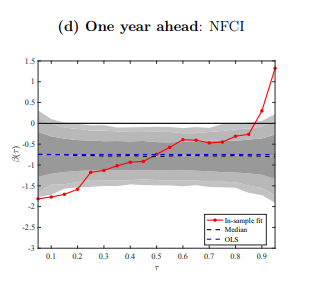
\includegraphics[width=0.5\textwidth]{Slides/Figures/abgqrnfci.png}
% % \end{figure}
% \begin{figure}[!htb]
%  \centering
%  {\scriptsize{NFCI and GDP growth  (Adrian et al., 2019)}}\\
%  \includegraphics[width=0.38\textwidth]{Slides/Figures/slope_nfci___Country=US___GDP=GDPG___SpecWith=gdp_nfci___Scenario=Baseline___Lags=0___Sample=1973-Q1_to_2015-Q4.pdf} \includegraphics[width=0.38\textwidth]{Slides/Figures/slope_gdp___Country=US___GDP=GDPG___SpecWith=gdp_nfci___Scenario=Baseline___Lags=0___Sample=1973-Q1_to_2015-Q4.pdf}

 
% \end{figure}

% \begin{figure}[!htb]
%  \centering
%  {\scriptsize{BAA-10-Year spread and GDP growth}}\\
%  \includegraphics[width=0.38\textwidth]{Slides/Figures/slope_baa10ym___Country=US___GDP=GDPG___SpecWith=gdp_baa10ym___Scenario=Baseline___Lags=0___Sample=1973-Q1_to_2015-Q4.pdf} \includegraphics[width=0.38\textwidth]{Slides/Figures/slope_gdp___Country=US___GDP=GDPG___SpecWith=gdp_baa10ym___Scenario=Baseline___Lags=0___Sample=1973-Q1_to_2015-Q4.pdf}

% \end{figure}
% \vspace*{-0.2in}
% \hyperlink{disadvantagesqr}{\beamerbutton{Back}}

% }


\subsection{Approximation Error}
\begin{frame}[noframenumbering,label={approxerrorabg}]
\thispagestyle{empty}
       \begin{center}
         \structure{\Huge {\color{black}{\insertsubsection}}}
       \end{center}
     \end{frame}

\frame{
\frametitle{Estimating PDFs from QR: Approximation Error}
\framesubtitle{From \citet{Adrianetal2019}}
\label{approxerrprabg}

\begin{figure}[!htb]
 \centering
 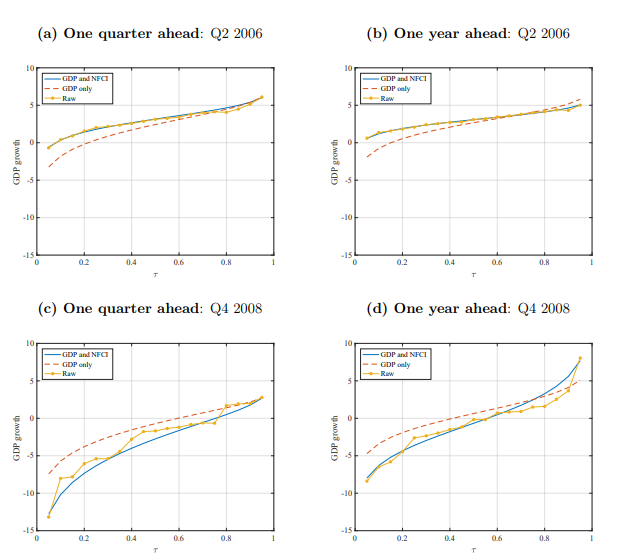
\includegraphics[width=0.67\textwidth]{Slides/Figures/approxerrorABG.png}
\end{figure}

\vspace*{-0.2in}
\hyperlink{azzintro}{\beamerbutton{Back}}

}


\section{Check Function}
\begin{frame}[noframenumbering]
\thispagestyle{empty}
       \begin{center}
         \structure{\Huge {\color{black}{\insertsection}}}
       \end{center}
     \end{frame}
     

\begin{frame}
\frametitle{Inspecting the Check Function \citep{koenker_2005}}
\label{checkfct}
  \vspace{0.25cm}
  \begin{itemize}
    \item Finding the $\tau$th quantile is a problem of \emph{ordering} sample observations, obtained as the solution to a simple \emph{optimization} problem.
        \bigskip
    \item Minimization problem
    \begin{equation*}
\min_{\theta_{\tau} \in \mathbb{R}^K} \sum_{t=1}^{T} \left(\tau \cdot \mathbbm{1}_{(y_{t}\geq x_t\theta_{\tau})} \lvert y_{t} - x_t \theta_{\tau} \rvert + (1-\tau) \cdot \mathbbm{1}_{(y_{t} < x_t \theta_{\tau})} \lvert y_{t} - x_t \theta_{\tau} \rvert \right)
\end{equation*}
can be rewritten as a linear program s.t. linear constraints.
  \end{itemize}
\begin{figure}[!htb]
 \centering
 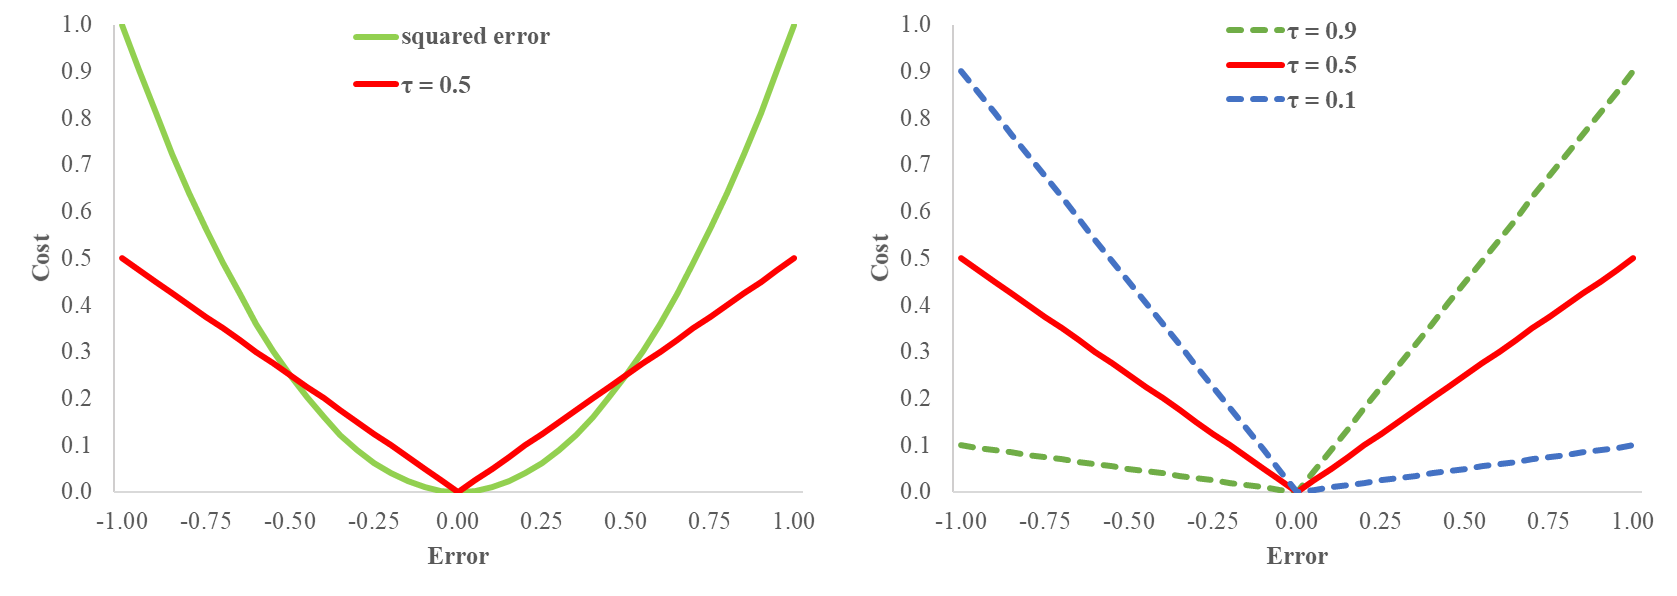
\includegraphics[width=0.75\linewidth]{Slides/Figures/quantile_reg_v2}
 \end{figure}
    \smallskip
    \hyperlink{qr}{\beamerbutton{Back}}
\end{frame}


\frame{
\frametitle{Trick is to Redefine the Residual Term}
  \vspace{0.25cm}
  \begin{itemize}
    \item Define $\epsilon_t = y_t - x_t\theta_t = u_t - v_t$, where
    \begin{eqnarray*}
    % \nonumber to remove numbering (before each equation)
      u_t &=& \mathbbm{1}_{(\epsilon_t \geq 0)} |\epsilon_t|\geq 0, \\
      v_t &=& \mathbbm{1}_{(\epsilon_t < 0)} |\epsilon_t|\geq 0. \\
    \end{eqnarray*}
  \item Minimization problem becomes
    \begin{equation*}
 \min_{\theta_{\tau} \in \mathbb{R}^K} \sum_{t=1}^{T} \left(\tau u_t + (1-\tau) v_t \right),
\end{equation*}
where the residuals must satisfy the $T$ constraints that
    \begin{equation*}
 y_t - x_t\theta = \epsilon_t = u_t - v_t.
\end{equation*}


  \end{itemize}

}


\frame{
\frametitle{Deriving the Linear Program}
  \vspace{0.25cm}
  \begin{itemize}
    \item This results in the linear program

    \begin{align*}
    &\min_{\theta_{\tau} \in \mathbb{R}^K, u \in \mathbb{R}^T, v \in \mathbb{R}^T} \sum_{t=1}^{T} \left\{\tau u_t +(1-\tau) v_t \right\}&\\
    s.t.\\
    &y_t - x_t\theta = u_t - v_t& \\
    &u_t \geq 0& \\
    &v_t \geq 0& \\
    \end{align*}
    which can be solved by interior point methods, among others.
    \bigskip
    \item[] \hyperlink{qr}{\beamerbutton{Back}}  

\end{itemize}


}

\subsection{Historical Data}
\begin{frame}[noframenumbering]
\thispagestyle{empty}
       \begin{center}
         \structure{\Huge {\color{black}{\insertsubsection}}}
       \end{center}
     \end{frame}


\frame{
\frametitle{Historical Data}
\label{Hist}

\begin{figure}[!htb]
 \centering
  \includegraphics[width=0.65\textwidth]{Slides/Figures/Data_US_FE___Sample=1986-Jan_to_2020-Apr.pdf}
%  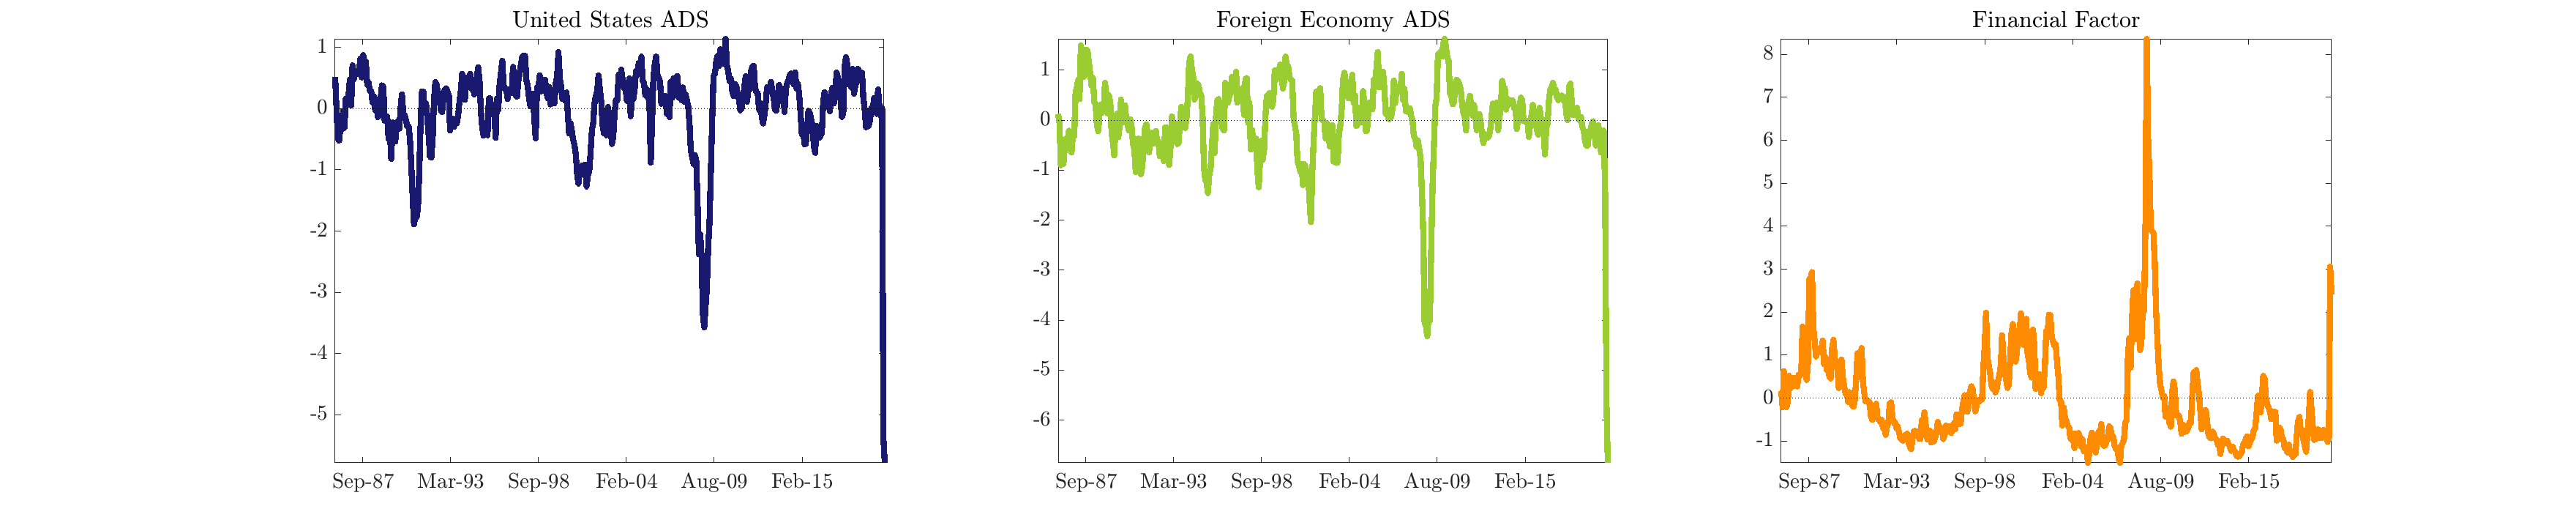
\includegraphics[width=1.05\textwidth]{Slides/Figures/graph_hist.png}
%   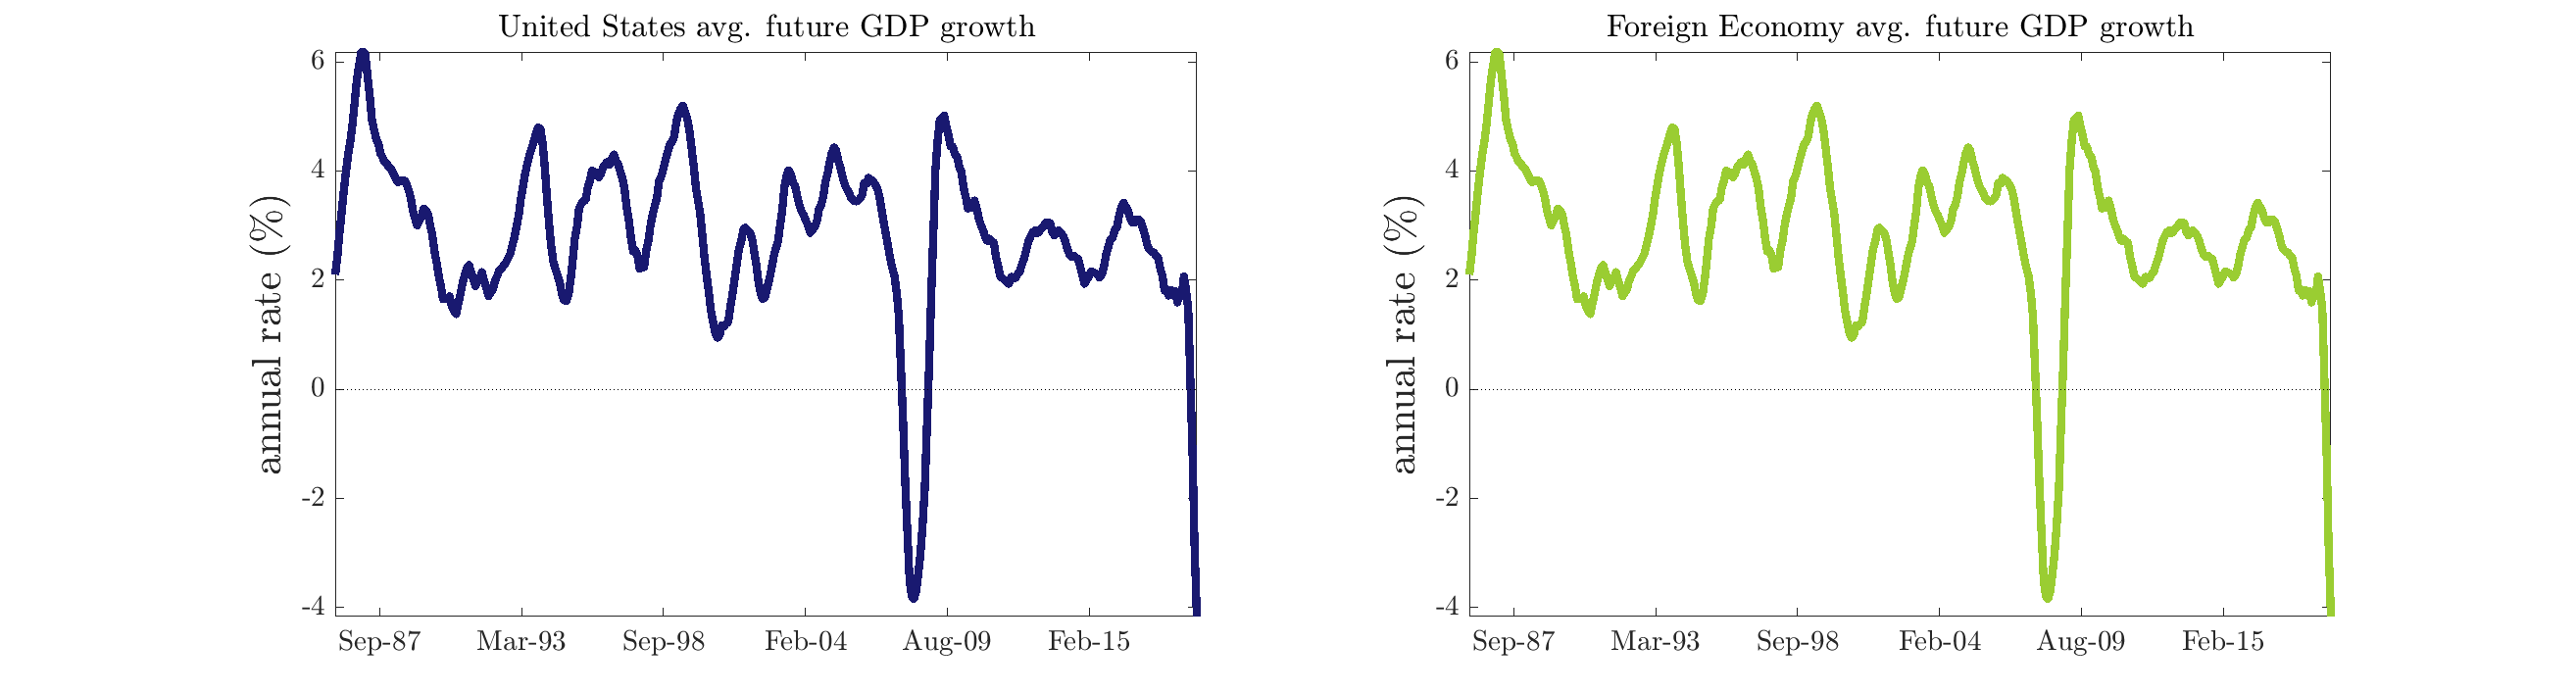
\includegraphics[width=0.85\textwidth]{Slides/Figures/graph_future_growth.png}
\end{figure}
\medskip
\hyperlink{modeldata}{\beamerbutton{Back (Model)}}
\hyperlink{condquant}{\beamerbutton{Back (United States)}}
\hyperlink{condquant_fn}{\beamerbutton{Back (Foreign Economy)}}
}



\subsection{Assessing Statistical Significance}
\begin{frame}[noframenumbering]
\thispagestyle{empty}
       \begin{center}
         \structure{\Huge {\color{black}{\insertsubsection}}}
       \end{center}
     \end{frame}



\frame{
\frametitle{Bootstrapping Techniques for Quantile Regressions}
\label{bootstrap}
\begin{itemize}
  \item \textbf{``Blocks-of-blocks''} bootstrap:
\medskip
\begin{enumerate}
  \item Divide the dependent variable $y$ and the regressors $X$ into $l$ consecutive blocks of all possible $m$-tuples.
  \medskip
  \item At each bootstrap replication, blocks of data are randomly drawn to form a new sample of the same size as the original data.
  \medskip
  \item Blocks are resampled in the same order for both the dependent variable $y$ and the regressors $X$, a key step which preserves the time-dependency in the data.
\end{enumerate}
\bigskip

\item Confidence intervals of bootstrapped coefficients' statistic $f(\beta_{b})$:
\medskip
\begin{enumerate}
  \item Generate statistic $f(\beta_{b})$ for each $b=1,\ldots,N_b$ bootstrap replicas.
  \medskip
  \item Construct percentiles of $f(\beta_{b})$ to obtain confidence interval.
\end{enumerate}
\end{itemize}

}


\frame{
\frametitle{``Blocks-of-Blocks'' Bootstrap Advantages}

\begin{itemize}
\item  Preserves crucial feature of quantile regression:\\ Agnostic about the underlying distribution of the error terms.
\bigskip
\item Maintains (time-series) dependency in the data, which would in most cases be destroyed by a naive bootstrap.
\bigskip
\item Used when a researcher is interested in computing confidence intervals around nonsymmetric statistics of the underlying data.
\bigskip
\item Relevant since our quantile regression model is a $h$-step predictive regression and slopes are non-linear functions of the data.
\bigskip
\item  See Chapter 12 of \citet{LutzHelmut2018} for more details.
\bigskip
\item[] \hyperlink{condquant}{\beamerbutton{Back}}
\end{itemize}

}


\frame{
\frametitle{Assessing Statistical Significance - United States}
\label{bootfullsample}

\begin{figure}[!htb]
 \centering
 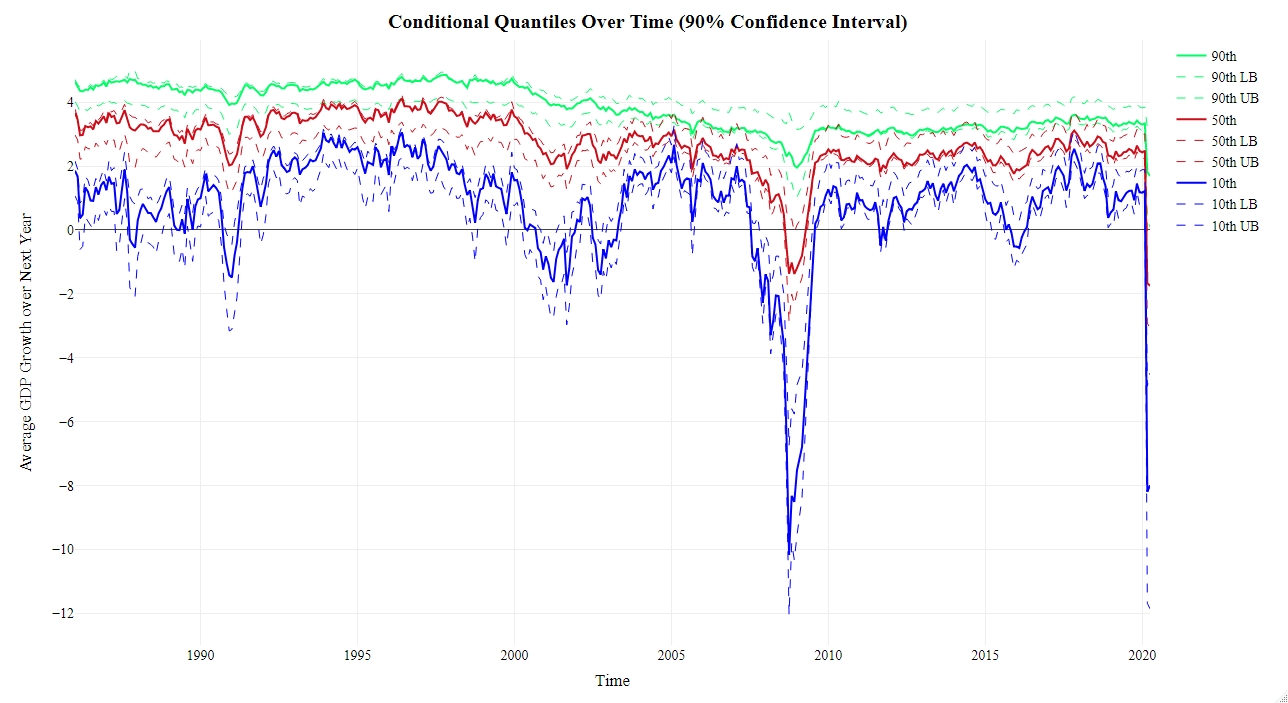
\includegraphics[width=\textwidth]{Slides/Figures/quantiles_boot}
\end{figure}
\hyperlink{condquant}{\beamerbutton{Back}}
}

\frame{
\frametitle{Conditional Quantiles over Time - United States}
\framesubtitle{Global Financial Crisis}
\label{bootGFC}

\begin{figure}[!htb]
 \centering
 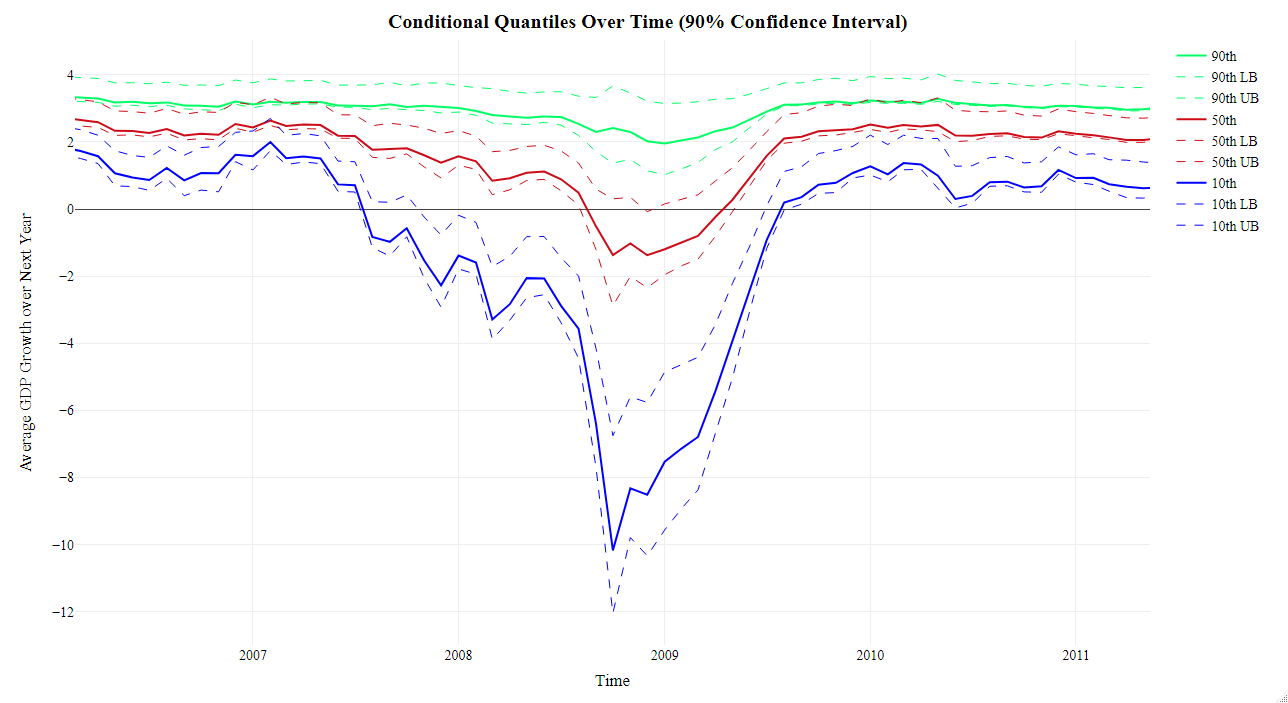
\includegraphics[width=\textwidth]{Slides/Figures/quantiles_boot_GFC}
\end{figure}
\medskip
\hyperlink{condquant}{\beamerbutton{Back}}
}



\frame{
\frametitle{Conditional Quantiles over Time - United States}
\framesubtitle{COVID-19 Outbreak}
\label{bootCOVID}

\begin{figure}[!htb]
 \centering
 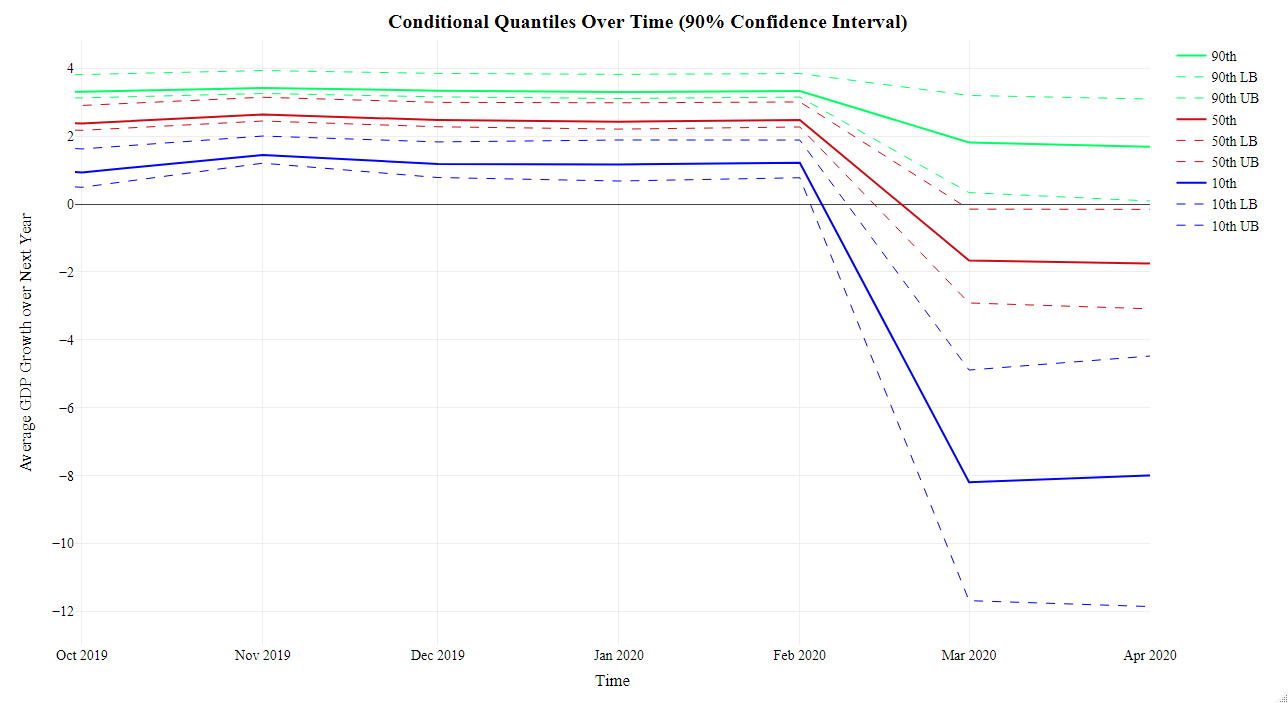
\includegraphics[width=\textwidth]{Slides/Figures/quantiles_boot_covid}
\end{figure}
\medskip
\hyperlink{condquant}{\beamerbutton{Back}}
}





\subsection{From Quantiles to Distributions\\ \bigskip \large A Step-by-Step Example}
\begin{frame}[noframenumbering]
\thispagestyle{empty}
       \begin{center}
         \structure{\Huge {\color{black}{\insertsubsection}}}
       \end{center}
     \end{frame}

% \frame{
% \frametitle{Obtaining the Time Series of Conditional Quantiles}
% \label{TSQSteps}
% \begin{itemize}

% \item At each point in time $t$, it is possible to use data on $FF_t$ and $ADS_t$ to construct $\hat{\text{Q}}_{\tau} (\Delta \bar{y}_{t+1,t+12}| x_t)$.
% \bigskip
% \item \rr{Example}: United States, April 2020, $FF=2.41$; $ADS-5.78$.
%   \bigskip
%   \item Coefficients for the $10th$ quantile are
%   \begin{equation*}
%     \hat{\alpha}_{\tau=0.1} = -1.72,\ \hat{\beta}_{\tau=0.1} = -0.95,\ \hat{\gamma}_{\tau=0.1} = 1.04
%   \end{equation*}
%   \item $10th$ Conditional quantile is: 
%   \bigskip
%   {\footnotesize
%     \begin{equation*}
%     \hat{\text{Q}}_{\tau=0.1} (\Delta \bar{y}_{20:m5,\ 21:m4}| x_{20:m4}) = -1.72 + (-0.95) \cdot 2.41 + 1.04\cdot (-5.78) + \underbrace{2.03}_{trend} = -7.99
%     \end{equation*}
%     }
%     \medskip
%   \item Construct similarly remaining  quantiles ($25th$, $50th$, $75th$, $90th$).\\[0.25cm] \hyperlink{linearqr}{\beamerbutton{Back}}
% % \bigskip
% % \item Important: $\hat{\text{Q}}_{\tau} (\Delta \bar{y}_{t+1,t+12}| x_t)$ is an \textbf{output} of the model.
% \end{itemize}

% }

\frame{
\frametitle{Obtaining the Time Series of Conditional Quantiles}
\label{TSQSteps}
\begin{itemize}

\item At each point in time $t$, it is possible to use data on $FF_t$ and $ADS_t$ to construct $\hat{\text{Q}}_{\tau} (\Delta \bar{y}_{t+1,t+12}| x_t)$.
\bigskip
\item \rr{Example}: Foreign Economy (TW), April 2020, $FF=2.41$; $ADS-6.85$.
  \bigskip
  \item Coefficients for the $10th$ quantile are
  \begin{equation*}
    \hat{\alpha}_{\tau=0.1} = -1.28,\ \hat{\beta}_{\tau=0.1} = -0.79,\ \hat{\gamma}_{\tau=0.1} = 0.55
  \end{equation*}
  \item $10th$ Conditional quantile is: 
  \bigskip
  {\footnotesize
    \begin{equation*}
    \hat{\text{Q}}_{\tau=0.1} (\Delta \bar{y}_{20:m5,\ 21:m4}| x_{20:m4}) = -1.28 + (-0.79) \cdot 2.41 + 0.55\cdot (-6.85) + \underbrace{1.84}_{trend} = -5.11
    \end{equation*}
    }
    \medskip
  \item Construct similarly remaining  quantiles ($25th$, $50th$, $75th$, $90th$).\\[0.25cm]
% \bigskip
% \item Important: $\hat{\text{Q}}_{\tau} (\Delta \bar{y}_{t+1,t+12}| x_t)$ is an \textbf{output} of the model.
\end{itemize}

}

\frame{
\frametitle{A Step-by-Step Example\\ \small Fitting the Skewed $t$-Distribution}
  \label{azzsbs}
\begin{itemize}
  \item In April 2020, the four quantiles to fit the distribution are:
  \begin{eqnarray*}
    &\hat{\text{Q}}_{\tau=0.10} (\Delta \bar{y}_{20:m5,\ 21:m4}| x_{20:m4}) &= -5.11,\\
    &\hat{\text{Q}}_{\tau=0.25} (\Delta \bar{y}_{20:m5,\ 21:m4}| x_{20:m4}) &= -3.09,\\
    &\hat{\text{Q}}_{\tau=0.75} (\Delta \bar{y}_{20:m5,\ 21:m4}| x_{20:m4}) &=  \phantom{+}0, \\
    &\hat{\text{Q}}_{\tau=0.90} (\Delta \bar{y}_{20:m5,\ 21:m4}| x_{20:m4}) &= \phantom{+}2.02,\\
  \end{eqnarray*}
  \item  Find distribution parameters ${\Theta}$ that minimize distance between:
  \begin{center}
      $\hat{\text{Q}}_{\tau=\{0.1,0.25,0.75,0.9\}}(\Delta \bar{y}_{20:m5,\ 21:m4}| x_{20:m4})$ from QR model and\\
  $F^{-1}_{\Delta \bar{y}}(\tau=\{0.1,0.25,0.75,0.9\}|x_{20:m4},{\Theta})$ from skewed $t-$distribution.
  \end{center}
  \bigskip
\item Density in April 2020 is skewed $t$-PDF $\ f(\Delta \bar{y}_{20:m5,\ 21:m4}|x_{20:m4},\hat{\Theta})$ constructed using estimated distribution parameters $\hat{\Theta}$.\smallskip
\end{itemize}
\hyperlink{azzintro}{\beamerbutton{Back}}
}


\subsection{Assessing the Correct Calibration of the Model}
\begin{frame}[noframenumbering,label={PITs}]
\thispagestyle{empty}
       \begin{center}
         \structure{\Huge {\color{black}{\insertsubsection}}}
       \end{center}
     \end{frame}


\frame{
\frametitle{A Formal Test\\ \small \cite{RossiSekhposyan2019}}

\begin{itemize}
  \item Test for correct calibration of the conditional predictive distributions implied by the quantile regression model.
  \bigskip
  \item \bb{Correct calibration}: Probability that the realized value is above or below the predicted value is the same (on average, across time) irrespectively of whether realizations are high or low.
  \bigskip
  \item The test evaluates the absolute predictive ability of a model at its estimated parameter values and, thus, in finite samples.
      \bigskip
  \item In this sense, both the parametric model and the estimation technique employed are being evaluated.
\end{itemize}

}


\frame{
\frametitle{How the Tests Works in Practice}

\begin{itemize}
\item Estimate the quantile regression model and construct out-of-sample conditional quantiles.
\medskip
\item Fit distribution on out-of-sample conditional quantiles.
\medskip
\item Back out quantile of realized value from predicted distribution, formally known as the probability integral transform (PIT):
    \begin{equation*}
    PIT_t \equiv Prob\left(\Delta \bar{y}_{t+1,t+12}<\Delta \bar{y}^*_{t+1,t+12}|x_t\right).
    \end{equation*}

\medskip

\item In a perfectly calibrated model, the predictive density should feature a CDF which is uniform, i.e., equal to the $45^{\circ}$ line.

\medskip

\item If the empirical CDF of the PITs falls outside of the 5\% critical values, the null hypothesis of correct calibration is rejected.
\end{itemize}

}



\frame{
\frametitle{Evaluating Correct Calibration of Our Model}

\begin{figure}[!htb]
 \centering
 \includegraphics[width=0.7\textwidth]{Slides/Figures/RS_OOS____Country=US___GDP=GDP___SpecWith=fin_ads___Scenario=Baseline___Lags=0___Detrended=false___Sample=1986-Jan_to_2020-Apr.pdf}
\end{figure}
\hyperlink{azzintro}{\beamerbutton{Back}}

}



% \subsection{Data \& Estimation}
% \begin{frame}[noframenumbering,label={Data}]
% \thispagestyle{empty}
%       \begin{center}
%          \structure{\Huge {\color{black}{\insertsubsection}}}
%       \end{center}
%      \end{frame}
     
% \frame{
% \frametitle{Data \& Estimation}
% \framesubtitle{From 'Growth At Risk Models for the U.S. and the Foreign Economy (2020)'}

% \begin{itemize}
%     \item Average GDP growth between months $t+1$ and $t+12$
%     \medskip
%     \item CBOE S\&P100 Volatility Index (VXO)
%     \medskip
%     \item Arouba Diebold Scotti country-specific indexes estimated using a dynamic factor model with mixed frequency data:
%     \smallskip
% \begin{itemize}
%     \item Annualized quarterly growth rates of {\rr{real GDP}};
%     \smallskip
%     \item Annualized monthly growth rates of retail sales;
%     \smallskip
%     \item Annualized monthly growth rates of industrial production;
%     \smallskip
%     \item The new export order component of the PMI survey;
%     \smallskip
%     \item Initial unemployment insurance claims (United States ADS only)
% \end{itemize}
% \medskip
% \item {\rr{Estimation Sample}}: 1986:m1 - 2019:m3.\\
% $\longrightarrow$ Last in-sample observation of future GDP growth in 2019:m3 based on data from 2019:m4 through 2020:m3.
% \end{itemize}

% \vspace*{0.2in}
% \hyperlink{linearqr}{\beamerbutton{Back}}
% }


% \subsection{AdvanDisadvantages}
% \begin{frame}[noframenumbering,label={alterfin}]
% \thispagestyle{empty}
%       \begin{center}
%          \structure{\Huge {\color{black}{\insertsubsection}}}
%       \end{center}
%      \end{frame}




\frame{
\frametitle{References}
\bibliographystyle{chicago}
\bibliography{qr}
}







\end{document}
